% !TeX spellcheck = en_US


\section{Problem 9}
Again, suppose that we have the following two reference patterns and their targets:
\vspace{5mm}

\[
\begin{array}{ccc}
	%	\centering
	\left\{ 
	p_1 = \left[
	\begin{array}{c}
		1 \\
		2
	\end{array}
	\right], t_1 = \left[-1\right]
	\right\} & 
	\left\{ 
	p_2 = \left[
	\begin{array}{c}
		-2 \\
		1
	\end{array}
	\right], t_2 = \left[1\right]
	\right\}
\end{array}
\]
\vspace{5mm}

The probabilities of vectors $p_1$ and $p_2$ are equiprobable, so that means $P_1 = P_2 = 0.5$.

\subsection{Question a}
In order to sketch the contour plot of the Mean Square Error performance, we ought to calculate the arguments of the quadratic function F(x). As we did on Problem8-Question \ref{Questionb}, with the help of Matlab we calculate the c,R,h and we get the following results\\

\begin{itemize}
	\item $R = \left[
	\begin{array}{cc}
		2.5 & 0 \\
		0 & 2.5 \\
	\end{array}
	\right]
	$
	\item $h = \left[
	\begin{array}{c}
		-1.5 \\
		-0.5
	\end{array}
	\right]
	$
	\item c = 1
\end{itemize}
and the MSE function is:
$F(x) = 1 - 3 \cdot w_{11} -w_{12} + 2.5 \cdot w_{11}^2 + 2.5 \cdot w_{12}^2$ \\

From the form of the equation we can understand that it is a circle with a center of $x^* = R^-1 \cdot h.$\\
By the Matlab code that i provided to calculate the F(x), we get the 2D and 3D contour plots of the MSE index as shown in figures \ref{fig:prob_9_2d} and \ref{fig:prob_9_3d}\\
\begin{figure}[H]
	\centering
	\begin{subfigure}{0.47\textwidth}
		\centering
		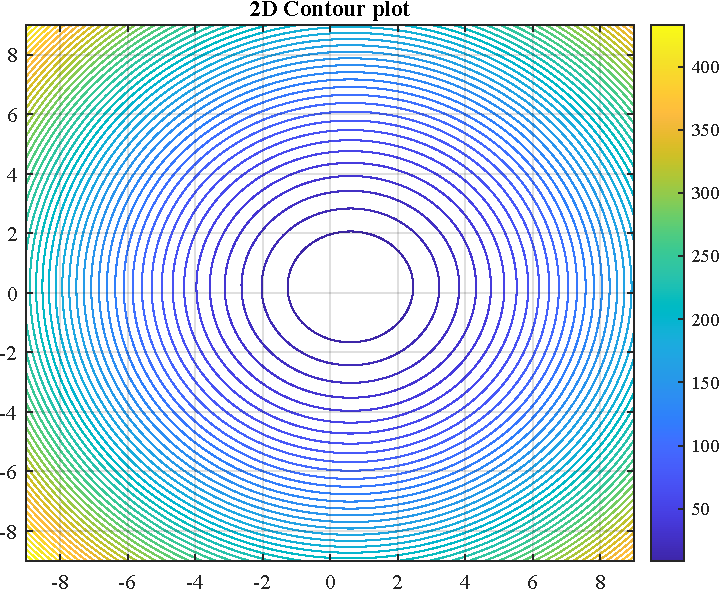
\includegraphics[width=\textwidth]{../Problem 9/contour_2d.pdf}
		\caption{2D plot of MSE index}
		\label{fig:prob_9_2d}
	\end{subfigure}
	\hspace{2mm}
	\begin{subfigure}{0.47\textwidth}
		\centering
		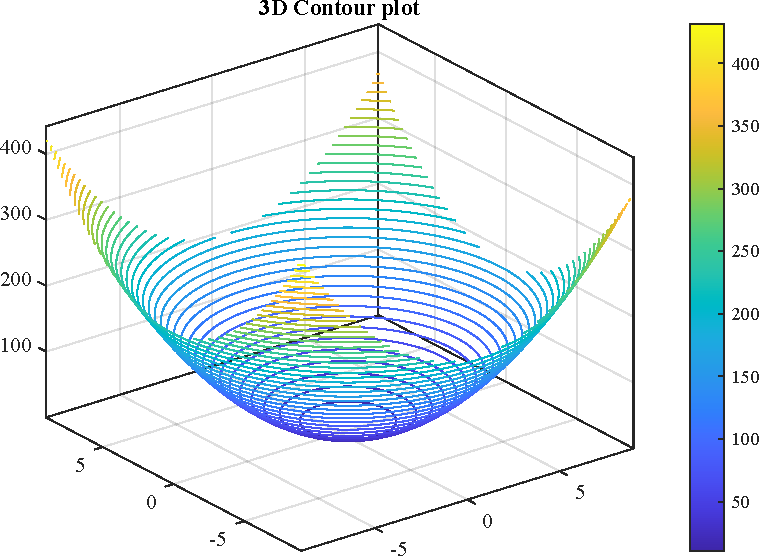
\includegraphics[width=\textwidth]{../Problem 9/contour_3d.pdf}
		\caption{3D plot of MSE index}
		\label{fig:prob_9_3d}
	\end{subfigure}	
\end{figure}

\subsection{Question b}
Working with the same method as i did in Problem8-Question \ref{Questionc} but this time with the help of Matlab code, we got the following sketch about the optimal decision boundary.

\begin{figure}[H]
	\centering
	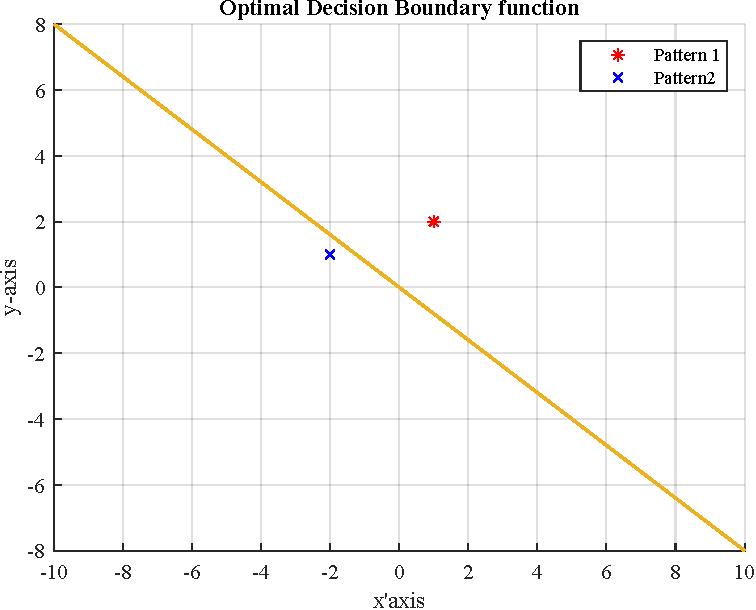
\includegraphics[width=0.5\textwidth]{../Problem 9/patterns.pdf}
	\caption{Optimal decision Boundary plot}
	\label{fig:OpDecBo}
\end{figure}

We can verify that indeed the optimal decision boundary separates and correctly classifies the patterns.

\subsection{Question c}
If we want to sketch the trajectory of the LMS algorithm on our contour plot, we follow the methodology of Problem8- Question\ref{Questione}, but for the number of iterations N = 100.\\
Here our learning rate is lr = 0.025 and the initial weight is $w(0) = \left[
\begin{array}{c}
	3 \\
	1
\end{array}
\right]
$

Using Matlab, we exported this trajectory of the LMS algorithm to our 2D contour plot of the mean square error performance index.
\begin{figure}[H]
	\centering
	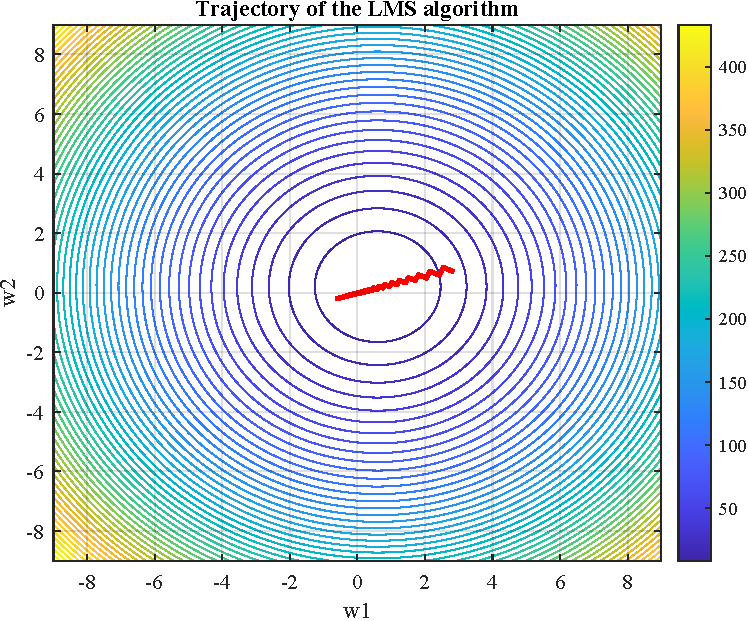
\includegraphics[width=0.45\textwidth]{../Problem 9/contour_2d_traj.pdf}
	\caption{Trajectory of the LMS algorithm}
	\label{fig:trajectory}
\end{figure}


